\documentclass[a4paper, 14pt]{extarticle}
\usepackage{float}
% Поля
%--------------------------------------
\usepackage{geometry}
\geometry{a4paper,tmargin=2cm,bmargin=2cm,lmargin=3cm,rmargin=1cm}
%--------------------------------------


%Russian-specific packages
%--------------------------------------
\usepackage[T2A]{fontenc}
\usepackage[utf8]{inputenc} 
\usepackage[english, main=russian]{babel}
%--------------------------------------

\usepackage{textcomp}

% Красная строка
%--------------------------------------
\usepackage{indentfirst}               
%--------------------------------------             


%Graphics
%--------------------------------------
\usepackage{graphicx}
\graphicspath{ {./images/} }
\usepackage{wrapfig}
%--------------------------------------

% Полуторный интервал
%--------------------------------------
\linespread{1.3}                    
%--------------------------------------

%Выравнивание и переносы
%--------------------------------------
% Избавляемся от переполнений
\sloppy
% Запрещаем разрыв страницы после первой строки абзаца
\clubpenalty=10000
% Запрещаем разрыв страницы после последней строки абзаца
\widowpenalty=10000
%--------------------------------------

%Списки
\usepackage{enumitem}

%Подписи
\usepackage{caption} 

%Гиперссылки
\usepackage{hyperref}

\hypersetup {
	unicode=true
}

%Рисунки
%--------------------------------------
\DeclareCaptionLabelSeparator*{emdash}{~--- }
\captionsetup[figure]{labelsep=emdash,font=onehalfspacing,position=bottom}
%--------------------------------------

\usepackage{tempora}

%Листинги
%--------------------------------------
\usepackage{listings}
\lstset{
  basicstyle=\ttfamily\footnotesize, 
  %basicstyle=\footnotesize\AnkaCoder,        % the size of the fonts that are used for the code
  breakatwhitespace=false,        % sets if automatic breaks shoulbd only happen at whitespace
  breaklines=true,                 % sets automatic line breaking
  captionpos=t,                    % sets the caption-position to bottom
  inputencoding=utf8,
  frame=single,                    % adds a frame around the code
  keepspaces=true,                 % keeps spaces in text, useful for keeping indentation of code (possibly needs columns=flexible)
  keywordstyle=\bf,       % keyword style
  numbers=left,                    % where to put the line-numbers; possible values are (none, left, right)
  numbersep=5pt,                   % how far the line-numbers are from the code
  xleftmargin=25pt,
  xrightmargin=25pt,
  showspaces=false,                % show spaces everywhere adding particular underscores; it overrides 'showstringspaces'
  showstringspaces=false,          % underline spaces within strings only
  showtabs=false,                  % show tabs within strings adding particular underscores
  stepnumber=1,                    % the step between two line-numbers. If it's 1, each line will be numbered
  tabsize=2,                       % sets default tabsize to 8 spaces
  title=\lstname                   % show the filename of files included with \lstinputlisting; also try caption instead of title
}
%--------------------------------------

%%% Математические пакеты %%%
%--------------------------------------
\usepackage{amsthm,amsfonts,amsmath,amssymb,amscd}  % Математические дополнения от AMS
\usepackage{mathtools}                              % Добавляет окружение multlined
\usepackage[perpage]{footmisc}
%--------------------------------------

%--------------------------------------
%			НАЧАЛО ДОКУМЕНТА
%--------------------------------------

\begin{document}

%--------------------------------------
%			ТИТУЛЬНЫЙ ЛИСТ
%--------------------------------------
\begin{titlepage}
\thispagestyle{empty}
\newpage


%Шапка титульного листа
%--------------------------------------
\vspace*{-60pt}
\hspace{-65pt}
\begin{minipage}{0.3\textwidth}
\hspace*{-20pt}\centering

\includegraphics[width=\textwidth]{emblem}
\end{minipage}
\begin{minipage}{0.67\textwidth}\small \textbf{
\vspace*{-0.7ex}
\hspace*{-6pt}\centerline{Министерство науки и высшего образования Российской Федерации}
\vspace*{-0.7ex}
\centerline{Федеральное государственное бюджетное образовательное учреждение }
\vspace*{-0.7ex}
\centerline{высшего образования}
\vspace*{-0.7ex}
\centerline{<<Московский государственный технический университет}
\vspace*{-0.7ex}
\centerline{имени Н.Э. Баумана}
\vspace*{-0.7ex}
\centerline{(национальный исследовательский университет)>>}
\vspace*{-0.7ex}
\centerline{(МГТУ им. Н.Э. Баумана)}}
\end{minipage}
%--------------------------------------

%Полосы
%--------------------------------------
\vspace{-25pt}
\hspace{-35pt}\rule{\textwidth}{2.3pt}

\vspace*{-20.3pt}
\hspace{-35pt}\rule{\textwidth}{0.4pt}
%--------------------------------------

\vspace{1.5ex}
\hspace{-35pt} \noindent \small ФАКУЛЬТЕТ\hspace{80pt} <<Информатика и системы управления>>

\vspace*{-16pt}
\hspace{47pt}\rule{0.83\textwidth}{0.4pt}

\vspace{0.5ex}
\hspace{-35pt} \noindent \small КАФЕДРА\hspace{50pt} <<Теоретическая информатика и компьютерные технологии>>

\vspace*{-16pt}
\hspace{30pt}\rule{0.866\textwidth}{0.4pt}
  
\vspace{11em}

\begin{center}
\Large {\bf Лабораторная работа № 4} \\ 
\large {\bf по курсу <<Разработка мобильных приложений>>} \\
\large <<Интеграция Яндекс.Карт>> 
\end{center}\normalsize

\vspace{8em}


\begin{flushright}
  {Студент группы ИУ9-71Б Баев Д.А \hspace*{15pt}\\ 
  \vspace{2ex}
  Преподаватель Посевин Д. П.\hspace*{15pt}}
\end{flushright}

\bigskip

\vfill
 

\begin{center}
\textsl{Москва 2023}
\end{center}
\end{titlepage}
%--------------------------------------
%		КОНЕЦ ТИТУЛЬНОГО ЛИСТА
%--------------------------------------

\renewcommand{\ttdefault}{pcr}

\setlength{\tabcolsep}{3pt}
\newpage
\setcounter{page}{2}

\section{Задание}\label{Sect::task}
Реализовать виджет Яндекс.Карт вывода объектов согласно варианта из
таблицы ниже, в виджете должна отображаться Яндекс.Карта с расположенными
на ней метками объектов, по клику на метку объекта должен открываться виджет с
подробной информацией об объекте.
\newpage
\section{Исходный код}

Исходный код программы представлен в листинге~\ref{lst:code1}

\begin{figure}[H]
\begin{lstlisting}[language={},caption={Реализация мобильного приложения},label={lst:code1}]
import 'package:flutter/material.dart';
import 'package:yandex_mapkit/yandex_mapkit.dart';
import 'package:dio/dio.dart';

void main() => runApp(MyApp());


class UserData {
  final String name;
  final String gps;
  final String address;
  final String tel;

  UserData({required this.name, required this.gps, required this.address, required this.tel});

  factory UserData.fromJson(Map<String, dynamic> json) {
    return UserData(
      name: json['name'] ?? '',
      gps: json['gps'] ?? '',
      address: json['address'] ?? '',
      tel: json['tel'] ?? '',
    );
  }
}

class MapPoint {
  final String name;


  /// Широта
  final double latitude;


  /// Долгота
  final double longitude;

  final String address;

  final String tel;

  const MapPoint({
    required this.name,
    required this.latitude,
    required this.longitude,
    required this.address,
    required this.tel
  });
}

class MyApp extends StatelessWidget {
  @override
  Widget build(BuildContext context) {
    return const MaterialApp(
      home: MapScreen(),
    );
  }
}

class MapScreen extends StatefulWidget {
  const MapScreen({Key? key}) : super(key: key);

  @override
  State<MapScreen> createState() => _MapScreenState();
}

class _MapScreenState extends State<MapScreen> {
  final Dio dio = Dio();
  late YandexMapController _yandexMapController;

  @override
  void initState() {
    super.initState();
  }

  Future<List<MapPoint>> fetchData() async {
    try {
      final response = await dio.get('http://pstgu.yss.su/iu9/mobiledev/lab4_yandex_map/2023.php?x=var23');
      if (response.statusCode == 200) {
        final List<dynamic> dataList = response.data;
        final List<UserData> userList = dataList.map((json) => UserData.fromJson(json)).toList();
        print(userList);
        List<MapPoint> points = [];
        for (var place in userList) {
          List<String> gps = place.gps.split(',').map((s) => s.trim()).toList();
          var xy = gps.map((s) => double.parse(s)).toList();
          var p = MapPoint(name: place.name, latitude: xy[0], longitude: xy[1], address: place.address, tel: place.tel);
          points.add(p);
        }
        return points;
      } else {
        throw Exception("Failed to load data");
      }
    } catch (e) {
      throw Exception(e);
    }
  }

  @override
  void dispose() {
    _yandexMapController.dispose();
    super.dispose();
  }

  @override
  Widget build(BuildContext context) {
    return Scaffold(
      appBar: AppBar(
        title: const Text("yandex"),
      ),
      body: FutureBuilder<List<MapPoint>>(
        future: fetchData(),
        builder: (context, snapshot) {
          if (snapshot.connectionState == ConnectionState.waiting) {
            return const CircularProgressIndicator();
          } else if (snapshot.hasError) {
            return Text('Error: ${snapshot.error}');
          } else {
            return YandexMap(
              onMapCreated: (controller) async {
                  _yandexMapController = controller;
                  await _yandexMapController.moveCamera(CameraUpdate.newCameraPosition(
                    const CameraPosition(target: Point(latitude: 50, longitude: 20), zoom: 3)
                  ));
              },
              mapObjects: getPlacemarkObjects(context, snapshot.data!),
            );
          }
        },
      ),
    );
  }

  List<PlacemarkMapObject> getPlacemarkObjects(BuildContext context, List<MapPoint> points) {
    List<PlacemarkMapObject> objects = [];
      int i = 0;
      for (var point in points) {

        print(point.name);
        print(point.address);
        var newObj = PlacemarkMapObject(mapId: MapObjectId(i.toString()),
            point: Point(latitude: point.latitude, longitude: point.longitude),
            opacity: 1,
            onTap: (_, __) => showModalBottomSheet(context: context, builder: (context) => _ModalBodyView(point: point))
        );
        objects.add(newObj);
        i += 1;
      }
      return objects;
  }
}

class _ModalBodyView extends StatelessWidget {
  const _ModalBodyView({required this.point});

  final MapPoint point;
  @override
  Widget build(BuildContext context) {
    return Padding(
      padding: const EdgeInsets.symmetric(vertical: 40),
      child: Column(mainAxisSize: MainAxisSize.min, children: [
        Text(point.name, style: const TextStyle(fontSize: 20)),
        const SizedBox(height: 20),
        Text(
          '${point.latitude}, ${point.longitude}',
          style: const TextStyle(
            fontSize: 16,
            color: Colors.grey,
          ),
        ),
        Text(point.address, style: const TextStyle(fontSize: 20)),
        Text(point.tel, style: const TextStyle(fontSize: 20))
      ]),
    );
  }
}


\end{lstlisting}
\end{figure}


\section{Результаты}

Результаты приведен на рисунках~\ref{fig:img1}-~\ref{fig:img3}

\begin{figure}[H]
\centering
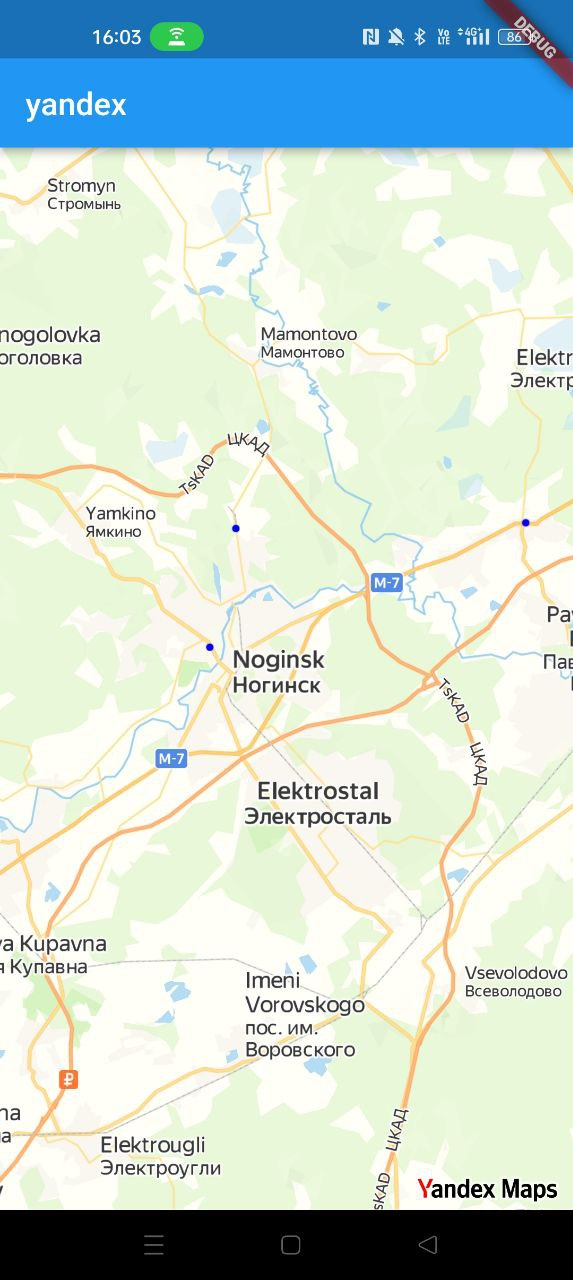
\includegraphics[width=0.5\textwidth]{images/res1.jpg}
\caption{Результат работы мобильного приложения}
\label{fig:img1}
\end{figure}

\begin{figure}[H]
\centering
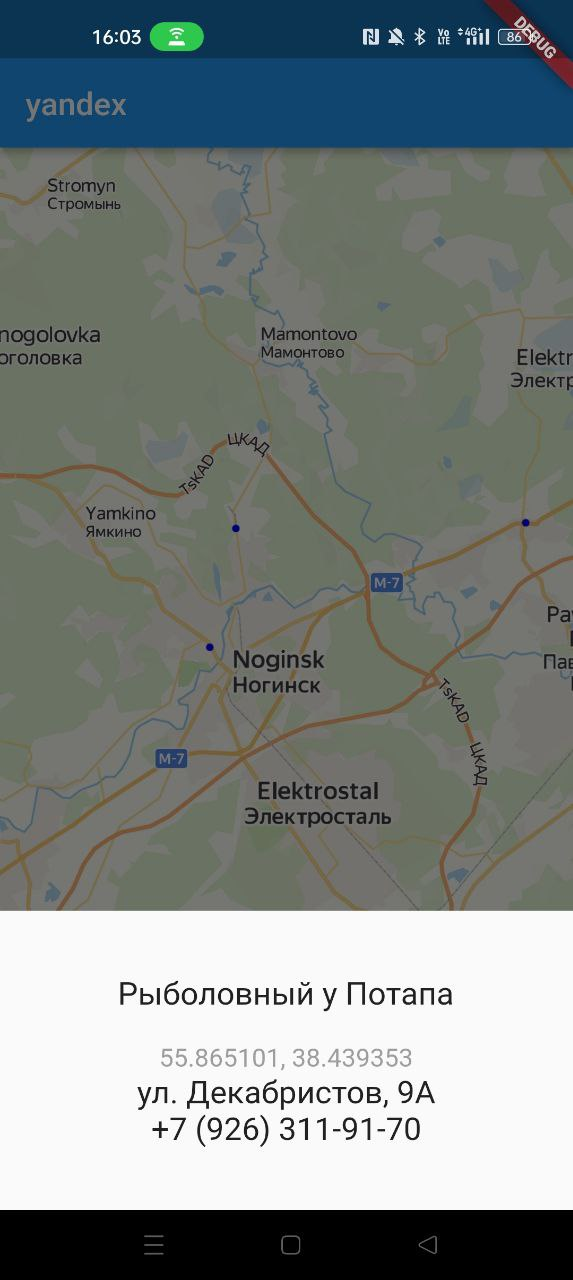
\includegraphics[width=0.5\textwidth]{images/res2.jpg}
\caption{Результат работы мобильного приложения}
\label{fig:img2}
\end{figure}

\begin{figure}[H]
\centering
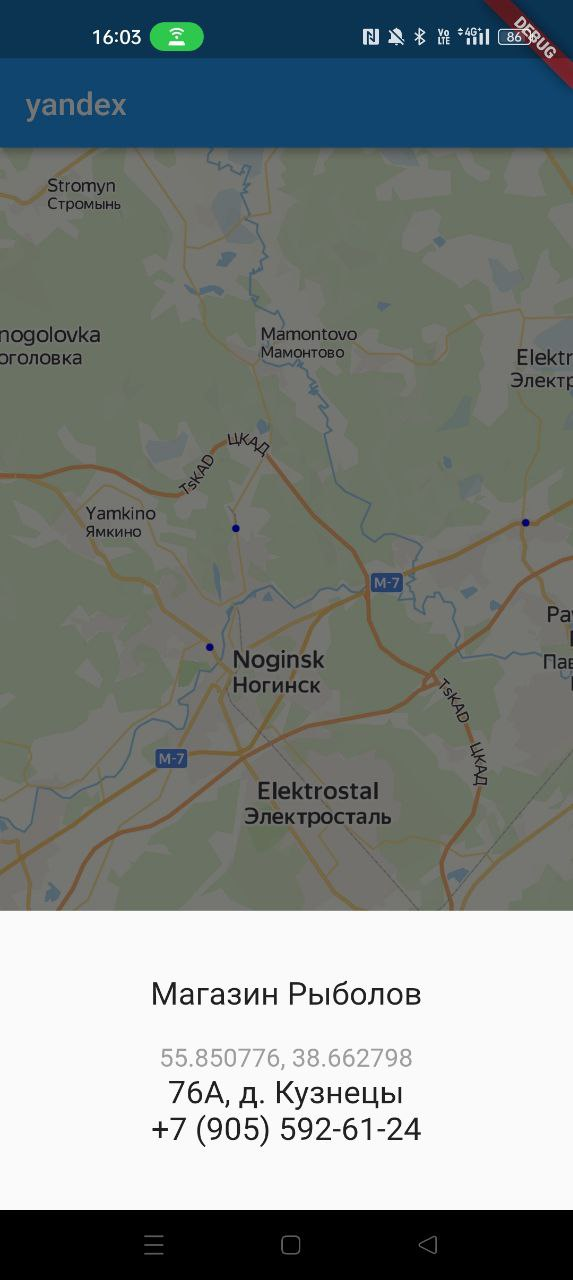
\includegraphics[width=0.5\textwidth]{images/res3.jpg}
\caption{Результат работы мобильного приложения}
\label{fig:img3}
\end{figure}


\section{Выводы}
В рамках данной лабораторной работы произошло знакомство с интеграцией с Яндекс.картами во flutter и установке меток на этих картах.
\end{document}
